\documentclass{beamer}
\usepackage{beamerthemeshadow}
\usepackage{graphicx}
\begin{document}
\title{Version control with git}
\author{Eike Mueller, University of Bath}
\date{\today} 

%%%%%%%%%%%%%%%%%%%%%%%%%%%%%%%%%%%%%%%%%%%%%%%%%%%%%%%%%%%%%%%%%%%%%%

\begin{frame}
  \frametitle{$ $}
  \titlepage
\end{frame}

%%%%%%%%%%%%%%%%%%%%%%%%%%%%%%%%%%%%%%%%%%%%%%%%%%%%%%%%%%%%%%%%%%%%%%

\begin{frame}
  \frametitle{Why version control?}
  \begin{center}
    
\includegraphics[width=0.5\linewidth]{phdcomics.png}
  \end{center}
  {\footnotesize ``Piled Higher and Deeper'' by Jorge Cham, \texttt{http://www.phdcomics.com}}
\end{frame}

%%%%%%%%%%%%%%%%%%%%%%%%%%%%%%%%%%%%%%%%%%%%%%%%%%%%%%%%%%%%%%%%%%%%%%

\begin{frame}
  \frametitle{Version control}
  \textbf{\Large What does it give us?}
  \begin{itemize}
  \item Systematic and controlled \textbf{Backup}
  \item \textbf{Collaborate}: work on same document simultaneously
  \item Keep track of changes (who introduced feature X and why?)
  \item \textbf{Try out changes} and \textbf{revert} to working version (``undo''-button)
  \item Work on project on \textbf{different machines}
  \item Simplifies \textbf{bug hunting}
  \end{itemize}
  \vspace{2ex}
  \textbf{\Large What's the catch?}
  \begin{itemize}
    \item Have to learn a few commands to interact with git
    \item Have to be organised
  \end{itemize}
\end{frame}

%%%%%%%%%%%%%%%%%%%%%%%%%%%%%%%%%%%%%%%%%%%%%%%%%%%%%%%%%%%%%%%%%%%%%%

\begin{frame}
  \frametitle{Applications}
  \textbf{\Large Version control can be be applied to:}
  \begin{itemize}
  \item \textbf{Source code} (matlab, Fortran, C, Python, \dots)
  \item \textbf{LaTeX} (your thesis!)
  \item Results
  \item \textbf{Any text files}\footnotemark
  \end{itemize}
  \footnotetext{Binary files work as well, but harder to track changes}
\end{frame}

%%%%%%%%%%%%%%%%%%%%%%%%%%%%%%%%%%%%%%%%%%%%%%%%%%%%%%%%%%%%%%%%%%%%%%

\begin{frame}
  \frametitle{Basic concepts}
  \begin{center}
    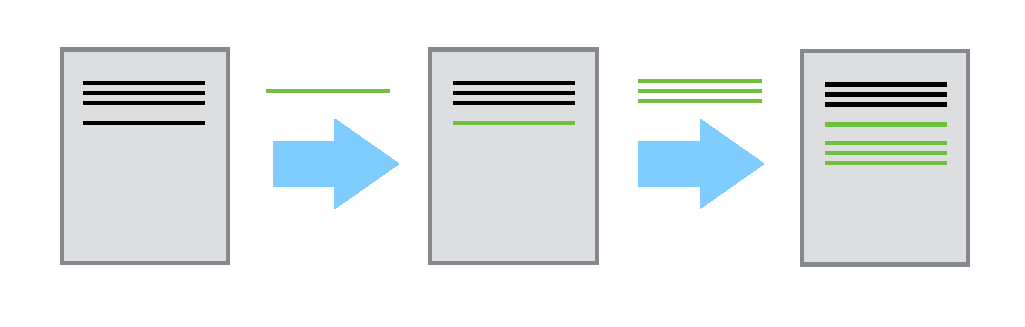
\includegraphics[width=0.6\linewidth]{play-changes.pdf}\\
    Tracking of changes
  \end{center}
  \begin{minipage}{0.45\linewidth}
    \begin{center}
      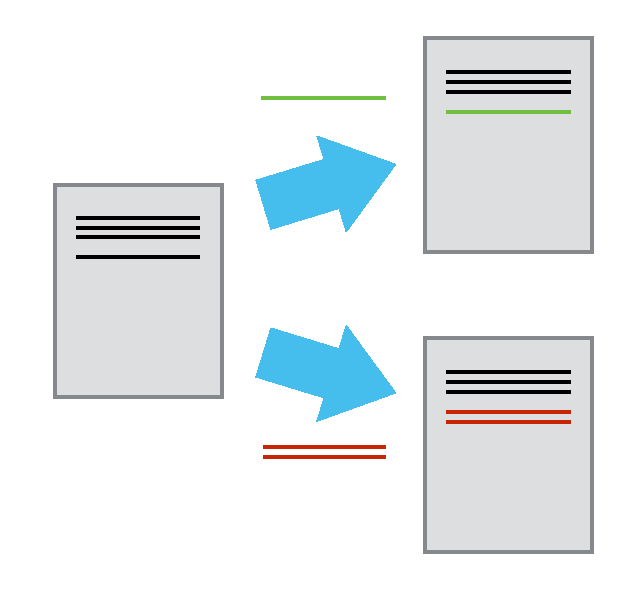
\includegraphics[width=0.6\linewidth]{versions.pdf}\\
      Collaborating
    \end{center}
  \end{minipage}
  \begin{minipage}{0.45\linewidth}
    \begin{center}
      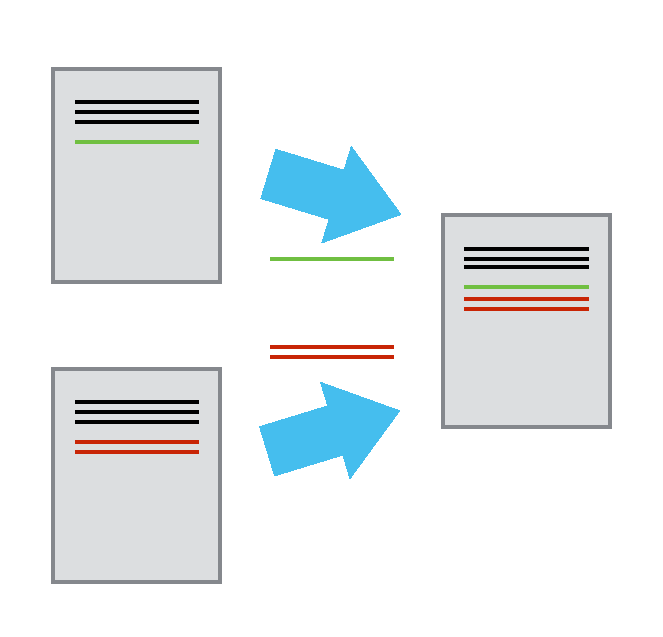
\includegraphics[width=0.6\linewidth]{merge.pdf}\\
      Merging and resolving conflicts
    \end{center}
  \end{minipage}\\[2ex]
  {\footnotesize All figures from Software Carpentry webpage}
\end{frame}

%%%%%%%%%%%%%%%%%%%%%%%%%%%%%%%%%%%%%%%%%%%%%%%%%%%%%%%%%%%%%%%%%%%%%%

\begin{frame}
  \frametitle{git}
  \textbf{\Large Why git?}
  \begin{itemize}
  \item \textbf{de-facto} standard now (supersedes subversion, CVS)
  \item Several nice features:
    \begin{itemize}
      \item Work remotely (distributed system)
      \item Simple and lightweight \textbf{branching}
      \item Selective commits (\textbf{staging} area)
      \item Very \textbf{powerful}
    \end{itemize}
  \item Not the easiest system to learn, so we'll only cover the basics
  \end{itemize}
  \vspace{2ex}
  \textbf{\Large Documentation}
  \begin{itemize}
  \item Git book: \texttt{http://git-scm.com/book/en/v2}
  \item Reference: \texttt{http://git-scm.com/docs}
  \end{itemize}
\end{frame}

%%%%%%%%%%%%%%%%%%%%%%%%%%%%%%%%%%%%%%%%%%%%%%%%%%%%%%%%%%%%%%%%%%%%%%

\begin{frame}
  \frametitle{Overview}
  \textbf{\Large Session 1} (Basics)
  \begin{itemize}
  \item Creating a git repository
  \item Tracking changes
  \item Exploring history
  \end{itemize}
  \vspace{2ex}
  \textbf{\Large Session 2} (Collaborating)
  \begin{itemize}
  \item Working with remotes (github)
  \item Collaborating and resolving conflicts
  \item Wrapup and advanced concepts (branching, merging, \dots)
  \end{itemize}
  \vspace{2ex}
  All material is based of Software Carpentry \texttt{http://git-scm.com/docs}
\end{frame}

\end{document}